% \vspace{2em}
% \pagebreak
\section{OS-level Page Access Obfuscation}
\label{sec:paging}
% \limcomm{I think we need a subsection for ORAM background because this section uses a lot of ORAM's terminologies, such as stash, leaf id, and position map. Reviewers without ORAM knowledge would not be able to understand this section.}{*}
\thename achieves OS-level page access obfuscation that operates independently from the \gls{gva} space.
\thename's paging subsystem maintains all CVM memory pages, including kernel and userspace pages (\reqfullsystem) as well as the \glspl{gpt}, in an ORAM-backed page pool and only allows memory accesses through a narrow and constantly rerandomized \gls{gpa} \emph{active regions}.
It carries out page-ins and page-outs in a page-access oblivious manner.
Also, it responds to the scheduler's rerandomization commands with eviction-based memory rerandomization to reshape the \gls{gpa} space.
% Nevertheless, \thename's paging operates transparently to the hosted program since it does not affect the gVA mappings for the hosted workload and the unikernel (\reqtransparent).
% \thename achieves OS-level transparency (\reqtransparent), which departs from prior approaches to runtime memory randomization~\cite{brasser2019drsgx} or access pattern obfuscation~\cite{ahmad2019obfuscuro, shinde2016preventing, zhang2020klotski} that require compiler instrumentation for software-based MMUs.
% \thename achieves transparency as an operating system (\reqtransparent), which departs from the previous approaches that for runtime memory randomization~\cite{brasser2019drsgx} or access pattern obfuscation~\cite{ahmad2019obfuscuro, shinde2016preventing, zhang2020klotski}, which typically require modifications to the program's virtual address layout itself through compiler instrumentation for software-based MMUs.


\begin{figure}[t]
	\centering
	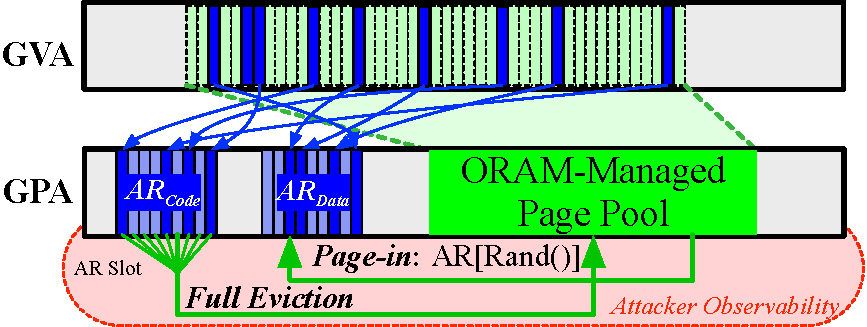
\includegraphics[width=.93\linewidth]{figures/incognitos/paging-overview-v4.pdf}
	\caption{\thename's system memory layout and page management}
	\label{fig:paging}
\end{figure}

\subsection{System memory layout}
\label{subsec:memory-layout}
The paging subsystem manages the following components to maintain the \thename system memory layout as shown in~\autoref{fig:paging}.
% \thename manages the following components to maintain \gls{cvm} page access obfuscation.

\iffalse
	\hdr{gVA-to-gPA mappings} The hosted program enjoys full freedom in laying out its components over the \gls{gva} space.
	The program's memory accesses through \gls{gva} are directed to randomized physical frame locations as in conventional operating systems, and \thename performs its constant rerandomization only in the \gls{gpa} space.
\fi

\label{subsec:oram-page-pool}
\hdr{ORAM-managed page pool}
% All \thename CVM pages are managed through an ORAM-managed page pool.
The page pool implements the Path ORAM scheme~\cite{stefanov2018path}, where each node is a page.
The path ORAM algorithm maintains a binary ORAM tree with height $l$ containing $N = 2^l-1$ buckets, each containing $Z$ blocks.
It also maintains an ORAM stash of $S$ in size to house fetched ORAM blocks temporarily.
An ORAM node may be a dummy page containing no actual data or a real page that stores the content of a memory page.

The Path ORAM algorithm performs data transfers between the ORAM tree and the ORAM stash at the granularity of \emph{paths} on the ORAM tree~\cite{stefanov2018path}.
It keeps a \gls{posmap} structure that maps each ORAM block to a randomized path indexed by the leaf nodes (\emph{leaf ID}).
In \thename, both the ORAM tree and stash are implemented as an array of pages in contiguous physical pages reserved during \gls{cvm} boot.
The ORAM \gls{posmap} is integrated with the OS page table, as described in \cref{subsec:paging-in-out}.
% \khacomm{mention leafID}{}



% All evaluations use the ORAM block size $B = 4KB$ (page size), bucket size $Z = 4$.

\iffalse
	Typically, ORAM metadata is stored alongside the block; however, since the size \thename's ORAM blocks are equivalent to a page, the metadata for ORAM needs to be maintained separately.
	\thename maintains metadata for the ORAM blocks in a shadow array, which will be accessed alongside the ORAM block, meaning that metadata and data have the same access pattern.
\fi



% \subsubsection{gVA-to-gGPA mappings}
% \key{The management of gVA-to-gPA mappings in \thename is performed through the \thename's custom \gls{vma} implementation that transparently enforces its ORAM-integrated page management (\cref{subsec:paging-in-out} and runtime memory rerandomization (\cref{subsec:rerand}) schemes
% (\reqtransparent).}
% During the boot process of the \gls{cvm}, \thename takes control over the unikernel virtual address space management for both kernel and userspace.
% It does this by replacing the existing management through \glspl{vma} with its own custom \glspl{vma} implementations.
% Additionally, for userspace addresses created through \texttt{mmap} system call, we also ensure they are backed by the \thename's \gls{vma}.
% This covers memory used by the trampolines used for \thename static binary instrumentation (\cref{subsec:tick-tramp-impl}).
% At runtime, \thename only changes the layout of the \gls{gpa} by constantly relocating physical pages, while the \gls{gva} address spaces remain unmodified after their initial setup.

% Its rerandomization leverage the pag
% \thename randomizes the layout of \gls{gpa} pages and then updates the \gls{gva}-to-\gls{gpa} address translation to reflect the new layout.
% \key{
%     Direct access to the MMU hardware, made efficient through the unikernel approach, allows for a \gls{gpa}-only memory randomization strategy that remains compatible with unmodified programs.
% } 


\label{subsubsec:active-regions}
\hdr{Active gPA regions}
\thename manages \gls{gva} address space and also the OS page table into the constrained and constantly randomized \emph{active gPA regions} (\actrg{Code} and \actrg{Data} in \autoref{fig:paging}).
\thename manages  \emph{separated regions} for \gls{cvm} code, data (including stack and heap), and page tables (\actrg{code}, \actrg{data}, and \actrg{pgt}).
This design decision is based on the fact that SEV SNP's hypervisor-side  \gls{npf} handler notifies the untrusted hypervisor of the type of \gls{pf}: code fetch, data fetch, and guest page table faults.
Hence, mixing the three types of pages in a smaller active gPA region does not increase security.
% \limcomm{I think we need new subsubsection for \emph{slots}}{*}

\hdr{Active region size}
Each active region can shelter a configurable number of \emph{slots} ($S$) of 4KB pages.
A slot may be \emph{occupied}, containing a page with an active mapping, or \emph{empty}.
Unlike previous work that prefers an active region (or scratchpad) that spans a single rerandomization unit or a small number of units~\cite{zhang2020klotski,obelix}, \thename chooses to acquire entropy through larger active regions (8,192 slots of 4KB per region), due to the known ciphertext weakness~\cite{li2021cipherleaks} of SEV-SNP.
We further discuss the issue in~\cref{sec:sec-analysis}.
% This is , the current development target of \thename. 
% We will discuss more the implications of this 

% \subsubsection{Entropy in active regions}
% \khacomm{Shorten, give pointer to security analysis}{.}
% \hjcomm{ciphertext}{Unlike previous work that prefers an active region (or scratchpad) that spans a single rerandomization unit or a small number of units, \thename opts for acquiring entropy through larger active regions.}
% During rerandomization, if a page is placed in the same slot by chance, the adversary can learn this information.
% Hence, \thename's approach is to have at least 8,192 slots (32MB) for each region to ensure the entropy.
%and we further discuss the issue in~\cref{sec:sec-analysis}.





\hdr{Isolated pages for inevitable disclosures}
\thename isolates certain kernel components whose locations are inherently exposed to the hypervisor into non-randomized address spaces to prevent information leakage.
For instance, the SEV-SNP architecture permits the hypervisor to inject faults/interrupts, allowing it to monitor \glspl{isr} and their subsequent execution.
When left on their original pages, these components may expose other code and data residing on the same page.
Such pages include pages containing explicit calls to the hypervisor (\texttt{vmgexit}), memory mappings for I/O, and \gls{isr} pages (including the OS \gls{pf} handler).
We further discuss the security of the \gls{pf} handler in \cref{subsec:security-discussion}.



% Explicit calls to the hypervisor (\texttt{vmgexit}) in I/O-related code and MMIO pages are such examples.
% Also, the \gls{isr} addresses are exposed as they are always executed immediately following a hypervisor-controlled interrupt.
% \limcomm{Redundancy}{Therefore, \thename isolates these components from their original locations} and \limcomm{Why?}{excludes them from rerandomization}.

% The interrupt and I/O-related code and data pages are such examples.
% Additionally, the addresses of I/O pages must be provided to the hypervisor for I/O operations.
% We isolate interrupt kernel components such as the \gls{isr} code/data and the \gls{idt} into a dedicated ELF section.
% For I/O pages, \thename also creates a dedicated section.


\subsection{Page management and randomization}
\label{subsec:paging-in-out}
% A summary of \thename's page management scheme is shown in \autoref{fig:paging}.
\thename maintains an ORAM-integrated page table that controls the mappings from \gls{gva} (guest virtual address) to \gls{gpa} (guest physical address) to regulate the \gls{cvm}'s memory access within the constantly randomized active regions.
As a result, the \gls{gva} remains unchanged after its initial setup.
Memory rerandomization and page management are performed using the \emph{page-in} and \emph{page-out} procedures, which obliviously transfer pages between the ORAM-managed page pool and the active regions.




\hdr{Integration of ORAM into OS page tables}
% \hjcomm{Need work}{\thename retrofits the unikernel's paging to integrate the ORAM-managed }
\thename's approach for coherently integrating ORAM into OS page tables is to essentially transform the \glspl{pte} themselves to function as the \gls{posmap} of the Path ORAM algorithms.
This eliminates the need to maintain a separate \gls{posmap} data structure.
\glspl{pte} in an \thename-managed page table may reside in one of three states: (1) \texttt{active}, where the encoded \gls{pfn} points to a region within the active regions or (2) \texttt{paged-out}, the backing page has been evicted to the ORAM page store, or (3) \texttt{unallocated}, which indicates that a new physical page frame must be allocated to support OS demand paging.
Specifically, for \texttt{paged-out} pages, \thename reuses \glspl{pte} of evicted pages to store their leaf IDs.
% eliminating the need for separate \gls{posmap} storage.
% \key{
%     \thename integrates ORAM into the OS page table through its ORAM leaf ID encoding scheme.}
%   Particularly, when paging out an \texttt{active} page, \thename encodes the ORAM leaf ID in \texttt{bits[51:12]} of its \gls{pte}, previously encoding the \gls{pfn}, before unsettling its \texttt{present} bit (\texttt{bit[0]}) and uses a dedicated bit  (\texttt{bit[9]}) to mark the page as \texttt{paged-out}.




\hdr{Page fault handling}
\thename's \gls{pf} handler is invoked when the MMU encounters any \gls{pte} with its present bit cleared (\texttt{paged-out} and \texttt{unallocated}).
It first performs a \emph{software} page table walk to identify the non-present \gls{pte}.
% The OS page fault handler is invoked \limcomm{hard to understand}{on memory access to a \gls{gva} page that has any \gls{pte} used for its translation in the non-present state (\texttt{page-out} and \texttt{unallocated}).}
% \thename's page fault handler first  
% \limcomm{??Redundnacy. How about: \thename's extended \gls{pte} }{\gls{pte} causing the page fault.}
For \texttt{unallocated} \glspl{pte},  the handler selects a random slot within the active region corresponding to the type of fault for its allocation (\actrg{Data} for read and write, and \actrg{Code} for execute, and \actrg{gpt} for page table faults).
% \limcomm{Too many \thename, How about \textbf{the pgf handler}}
If the chosen slot is occupied, the existing page is evicted through the page-out process.
Page-ins occur upon \glspl{pf} on \texttt{paged-out} PTEs, and the corresponding page is fetched from the ORAM-managed page pool into the active region.

% is triggered \limcomm{Hard to understand, when the page-ins are triggered?}{for \texttt{paged-out} PTEs to obliviously fetch the page from the ORAM page pool into the active region.}
% For \texttt{page-out}


\hdr{Page-In}\label{subsubsec:page-in}
The page-in process begins with a Path ORAM path fetch that retrieves pages based on the ORAM leaf ID in the \gls{pte} and moves them to the ORAM stash~\cite{stefanov2018path}.
A slot within the active region according to the type of fault is then randomly chosen as the \gls{gpa} for the paged-in page, similar to the handling of \texttt{unallocated} \glspl{pte}.
The page corresponding to \gls{pte} is then copied from the stash into the chosen slot.
This page is identified using the faulting \gls{gva} (e.g., \texttt{0xff..cc000}) and the page level where the \gls{pte} resides (e.g., PD or PT), which is stored as the page's ORAM metadata.
Since the ORAM stash resides in untrusted memory, to obscure which page is being fetched from the stash, \thename utilizes an oblivious memory access wrapper adapted from previous work~\cite{obelix}.
The wrapper ensures that all physical pages in the stash are touched, regardless of the target page.
% slot using vectorized instructions (e.g., \texttt{\_mm256\_blendv\_epi8}).




\label{subsubsec:page-out}
\hdr{Page-Out}
Page-outs occur on two occasions: (1) to serve the rerandomization scheme described next and (2) when the random slot for page allocation is occupied.
On a page-out, the target page is first written to the ORAM stash, where it will eventually return to the ORAM tree through ORAM shuffling.
ORAM algorithms utilize both real and dummy nodes.
Since the stash is stored in untrusted memory, the location of dummy slots must be protected to maintain ORAM's security guarantees~\cite{zhang2020klotski}.
To address this, \thename's stash implementation adopts a modified \texttt{WriteStash} operation from previous work~\cite{zhang2020klotski}.
It keeps track of the last stash slot written to, incrementing this index with each write to the stash.
When new pages (dummy or real pages) are to be added to the stash, an unused stash slot is selected starting from this index, resulting in an always-increasing write access pattern.
If no slots are available, the stash is reshuffled by compacting real blocks to the beginning using the oblivious memory wrapper, after which the empty slot index is reset.
Finally, the page's corresponding \gls{pte} is then encoded to be \texttt{paged-out}.
% which would trigger a page-in upon the page's next access.

% As noted by \cite{zhang2020klotski}, the positions of \hjcomm{never mentioned before}{dummy} and real blocks within the stash may be exposed through writes to the stash, which requires special hardening.
% For example, if a stash slot is written twice without ORAM eviction, it could indicate that it previously contained a dummy ORAM block.

% When new pages (dummy or real pages) are to be written into the stash (either during active region eviction or ORAM path fetching), a new empty stash slot is selected from this index, starting toward the end of the stash. 
% If there are no available new slots, the stash is reshuffled by obliviously compacting the real stash blocks to the beginning of the stash with the oblivious memory wrapper described previously.
% After this process, the last stash slot index is reset to the first dummy slot.

% \subsubsection{\hjcomm{Rewritten}{NPF-on-GPT information leak}}
\hdr{Rerandomization through full eviction}
\thename's paging subsystem performs eviction-based rerandomization upon receiving a request from the scheduler.
When rerandomization is to be performed, the paging subsystem evicts \emph{all} currently occupied slots within the active regions back to the ORAM-managed page pool.
Thus, memory accesses that follow the rerandomization would automatically construct randomized memory layouts through the oblivious and random page-in process.
% , and non-PGT \gls{gpa} addresses are constantly rerandomized by \thename.
% An NPF-on-GPT on a \gls{pte} at {\tt 0xa\textbf{b}000} signifies access to another distinct set of 512 pages (assuming two sets do not share an aliased page).


\hdr{Inclusion of page tables in rerandomization}
To maintain the obfuscation of the entire system (\reqfullsystem), \thename incorporates the \gls{gpt} into the rerandomization scheme.
Although this design choice adds non-trivial complexities, we must address the \gls{npfongpt} information leak we have identified.
Specifically, while an untrusted hypervisor has no direct source to leak \gls{gva} accesses, exposed \glspl{gpfn} of the \glspl{gpt} themselves can serve as an alternative identifier for the 4KB pages they map.
For instance, if there is a \gls{npfongpt} on one of two \glspl{pte} located at \gls{pfn} {\tt 0xa{\underline{a}}000} and {\tt 0xa{\underline{b}}000}, it means that a memory access to a specific set of 512 4KB pages is imminent.
As a result, the adversary can leak the \gls{gva} access pattern of the CVM execution with up to 2MB (4KB$\times$512) granularity by exploiting \glspl{pte} location leaks.

% Since accesses to higher-level page tables (PML4, PDPT) would only leak extremely coarse-grained information that is hardly useful to attackers, 

% \limcomm{Can be shortened}{*}
% \thename focuses its randomization efforts on the last two levels (PD and PT).
Since access to higher-level \glspl{gpt} (PML4, PDPT) would only leak extremely coarse-grained information, we focus on the last two levels (PD and PT).
% that could reveal actionable insights about the \gls{gva} access patterns.
% \limcomm{Can be shortened}{*}
\thename places each layer of the \gls{gpt} in a dedicated active region (e.g., \AR{gpt}{PT},\AR{gpt}{P\hspace{-0.1em}D}), such that their rerandomization may be performed independently.
% \limcomm{Can be shortened}{*}
To respect the dependencies between pages and their corresponding \gls{pte}, \thename's page evictions are performed in the reversed order of the \gls{gpt} hierarchy.
That is, page evictions are performed in the order of \actrg{Code}, \actrg{Data} first, then \AR{gpt}{PT} and finally \AR{gpt}{P\hspace{-0.1em}D}.


% We first explain the \gls{npfongpt} information leak that motivated \thename's decision to include page tables in its randomization scheme.
% which aims to randomly permutate the current \gls{gpa} page layout within the active regions while preserving the \gls{gva} space.
% To achieve a full-system memory rerandomization, \thename discards the currently active \gls{gpa} spaces (i.e., active slots in active regions) with the page-out mechanism.

% That is, page evictions are performed in the order of \actrg{code} and \actrg{data}, then \actrg{gpt}.
% \key{
% \thename's rerandomization scheme must also handle the dependencies between normal pages and their corresponding page tables pages.
% }
% \thename places each layer of the page table in a dedicated active region (e.g., $\mathcal{AR}_{gpt}^{PT}$, $\mathcal{AR}_{gpt}^{PD}$), such that their rerandomization may be performed independently.
% Then, when a rerandomization is to be performed, page evictions are performed in the reversed order of their level in the hierarchy.

\iffalse

	% Using this information, the hypervisor learns the cause of the fault (e.g., instruction fetch or MMU page table walk) and the \gls{gpa}.
	% The VMCB is not encrypted even when CVM mode is enabled for the guest VM~\cite{li2021cipherleaks}.

	% Even when \thename constantly rerandomizes the \gls{gpa} address space, this NPF-on-GPT may allow the adversary to profile the CVM's \gls{gva} space.
	% Assume that the adversary launches the conventional \gls{npf}-based page profiling attack while specifically looking for NPF-on-GPTs to collect the \glspl{gpa} of the page tables.



	% More specifically, the memory accesses performed on a page walk leads to \gls{gpa} access sequences ${GPA_{pml4}, GPA_{pdpt}, GPA_{pd}, GPA_{pt}}$ that could be used to fingerprint the \gls{gva} being translated.
	% For example, page table walks for the translation of two \glspl{gva} \texttt{0xa00000} and \texttt{0xb00000} will access the same $GPA_{pml4}$, $GPA_{pdpt}$, $GPA_{pd}$, but perform different $GPA_{pt}$ accesses.

	% While \thename's memory randomization scheme obscures the \gls{cvm}'s \gls{gpa} memory layout we found that a malicious hypervisor can still infer \gls{gva} access patterns by observing the sequence of page table accesses during address translation.
	% This weakness stems from the fact that even with randomized \glspl{gpa}, the hierarchical structure of page tables creates distinctive access patterns that reveal information about the underlying \gls{gva}.
	% An address translation through page table walk is performed by the hardware MMU on a TLB miss (may be induced by the hypervisor~\cite{amd64}) or by the OS page fault handler to handle a \gls{gva} fault.

	% By leveraging the \gls{npf} controlled channel, the attacker can trace the sequence of page table accesses during this process, yielding a distinct signature that \hjcomm{??}{betrays} the \gls{gva} being translated.



	% Note that the eviction of page tables must follow specific constraints, as we will discuss in \cref{subsec:pgt-rerand}.


	\hdr{Page tables-specific rerandomization considerations}
	The \gls{npfongpt} leak calls for the inclusion of the page tables in the rerandomization scheme.
	% Memory accesses during page table walks at different levels reveal \gls{gva} access patterns at varying granularities: 256TB for PML4, 512GB for PDPT, 1GB for PD, and 2MB for PT level accesses.
	Since accesses to higher-level page tables (PML4, PDPT) would only leak extremely coarse-grained information that is hardly useful to attackers, \thename focuses its randomization efforts on the last two levels (PD and PT) that could reveal actionable insights about the \gls{gva} access patterns.

	\thename's rerandomization scheme must also handle the dependencies between normal pages and their corresponding page table pages.
	\thename places each layer of the page table in a dedicated active region (e.g., $\mathcal{AR}_{gpt}^{PT}$, $\mathcal{AR}_{gpt}^{PD}$), such that their rerandomization may be performed independently.
	Then, when a rerandomization is to be performed, page evictions are performed in the reversed order of their level in the hierarchy.
	That is, page evictions are performed in the order of \actrg{code}, \actrg{data} first, then $\mathcal{AR}_{gpt}^{PT}$ and finally $\mathcal{AR}_{gpt}^{PD}$.
	This ensures that all of the mapped pages are evicted before the page that maps them.
	% Since our rerandomization scheme completely evicts the active regions for rerandomization, all dependencies are evicted before their dependent.

	Similarly, random page replacement due to \textbf{page-ins} (\cref{subsubsec:page-in}) must also respect the page dependencies.
	Since only a limited number of page tables are active at a given time, conflict rarely occurs.
	However, on such occasions, we check if the existing page table contains active mappings by scanning its \glspl{pte} and selecting another random slot if it does.
\fi

% which ensures that all the dependent pages are evicted before the dependent page.






% \hjcomm{No idea what this means. Also too weak while the attack is explained in detail}{To maintain the integrity of address translation while randomizing page tables, \thename must respect the page table hierarchy. This hierarchical constraint drives the eviction sequence: first, \thename evicts data and code from active regions, then proceeds to evict page tables from the scratchpad in reverse hierarchical order - starting with PT pages before moving to PD pages.}


\iffalse
	\subsection{\hjcomm{Not too important. Can be killed for length}{Optimizations}}
	\label{subsec:pgt-optimizations}
	\thename also introduces several optimizations to efficiently manage page table pages through an ORAM page pool and avoid unnecessary complexities.

	% \subsubsection{Fast gVA-to-ORAM mapping}
	First, when a \gls{gva} fault occurs, \thename efficiently determines the corresponding ORAM block ID by combining the faulting address (from CR2) with the page table level where the non-present \gls{pte} is located.
	The following formula ensures a unique ORAM block ID $b$ for each \gls{gva} fault at any page table level:

	\vspace{0.5em}
	{
		$b = fault\_vaddr \land \lnot(2^{12 + 9\times page\_level} - 1) \oplus page\_level$
	}

	% \subsubsection{Repurposed PTEs for position map}
	Second, \thename reuses \glspl{pte} of evicted pages to store their ORAM leaf IDs, eliminating the need for separate position map storage.
	This also enables a recursive ORAM-like scheme where position map data for lower-level page tables is retrieved through successive ORAM fetches~\cite{freecursiveoram}.

	% \subsubsection{Integrated ORAM page walks}
	Lastly, rather than handling each page table fault separately, \thename enhances the OS page table walk to perform all necessary ORAM operations in a single pass. As the walk traverses each level reading \glspl{pte}, it automatically fetches ORAM-managed pool pages into active regions, eliminating the need for multiple separate \glspl{pf}.
\fi




% A suitable slot number may vary for each program;
% we set active region based on the empirically-observed working set page count, i.e., number of distinct pages that have been accessed at least once during runtime.
% For example, NGINX showed around 500 pages as its working set during maximum load, and we set it to be the slot count of its code active region.
% \khacomm{added}{
% The number of slots (i.e., $S$) is set to be at least \emph{twice} the \gls{cvm} \emph{immediate} working set between the normal rerandomization frequency \freqrrof{Normal}.
% For instance, we found that our evaluation targets NGINX's executable uses at the maximum of about 500 pages when \freqrrof{Normal} is $500,000$, so $S$ is chosen to be $1024$.
% This decision is influenced by our rerandomization mechanism, which performs full eviction of the active regions (\cref{subsec:rerand}).
% This strategy ensures that at least $50\%$ of the pages remain empty, so that the random page-in process (\cref{subsubsec:page-in}) does not introduce significant overhead.
% }

% throughout its execution.

% For instance, our evaluation target NGINX's executable contains \textcolor{red}{XX
% } code pages, and we configured the \actrg{code} to have \textcolor{red}{YYY} slots and \textcolor{red}{ZZZ} dummy pages have been added to the page pool as a result.
% than the total number of CVM pages ($N$) mapped into the region where $S - N$ dummy pages exist.


% This action causes every page in the \gls{cvm}'s working set to enter the \texttt{paged-out} state, leading to page-ins on their accesses.


% \subsubsection{Hardened Stash Implementation}
% \label{subsec:paging:hardenstash}
% Unlike the traditional threat model for Path ORAM, the stash must reside in untrusted memory in \glspl{cvm}, which introduces additional considerations.
% Specifically, two sources of leakage that could benefit attackers need to be eliminated. 



% \subsubsection{Physical memory (re)randomization scheme}
% \label{subsec:rerand}
% \label{subsec:pgt-rerand}
% \thename's paging subsystem performs eviction-based rerandomization upon receiving a request from the scheduler, which aims to randomly permutate the current \gls{gpa} page layout within the active regions while preserving the \gls{gva} space.
% \key{\thename's paging and rerandomization scheme also includes the page tables as a target of its memory rerandomization.}
% While this design decision introduces non-trivial complexity into the design, we found that this is indispensable for security due to an attack that may leak \gls{gva} layout through \glspl{npfongpt} (\reqfullsystem).


% Consequently, when the CVM attempts to access pages within its working set, a page fault is triggered, leading to page-ins.





% \key{
%     As a result of the combination of complete eviction and ORAM-protected page-ins, \thename achieves a new memory layout for the \gls{cvm} working set that is statistically independent of the previous one.
%     Moreover, thanks to ORAM protection, paged-in pages are unidentifiable when the memory accesses are observed, making the new randomized page layout secure.
% }


% \key{
%     The goals of \thename's memory rerandomization, especially when combined with the rate-adaptive policy (\cref{subsec:rerand-policy}), are twofold: (1) to significantly complicate the identification of sensitive pages through \gls{npf} page access profiling, and (2) to transform sensitive pages into moving targets that require considerable effort to track.
% }







% \key{During rerandomization, a random percentage number between 50\% to 100\% is chosen to decide the number of pages to be evicted.}


% During the page-in process, the Path ORAM algorithm ensures that the physical locations accessed in the page pool are indistinguishable from random accesses.
% This 






% \subsection{Page tables rerandomization}


% \key{\thename also identifies and mitigates a \emph{\gls{gva}} information leak in the current SEV-SNP implementation.}
% we discovered a source of an indirect \gls{gva} information leak through the page table locations in the \gls{npf} handling in SEV-SNP.
% \key{This weakness of SEV-SNP presents another non-trivial design requirement for \thename: the CVM page tables must also be constantly  rerandomized along with other pages.}



% \gls{gva} is never meant to be disclosed to the untrusted hypervisor in SEV-SNP's design, and hence \thename obfuscates the hypervisor-visible \gls{gpa} space.
% However,
% The information leak occurs during \glspl{npf} that occur on the guest CVM's (guest) page tables, and hence the name \emph{NPF-on-GPT}.
